\section*{2.2 矩阵}
\addcontentsline{toc}{section}{2.2 矩阵}
\label{sec:2.2}

矩阵在线性代数中起着核心作用。 它们可用于紧凑地表示线性方程组，此外它们也表示线性函数（线性映射），我们将在后面的2.7节中看到。 在我们讨论这些有趣的话题之前，让我们首先定义矩阵是什么以及我们可以对矩阵进行什么样的操作。 我们将在第4章看到更多矩阵的性质。

\textbf{定义 2.1} （矩阵）。对于 $ m,n \in \mathbb{N} $，实值 $ (m,n) $ \emph{矩阵（matrix）} $ \boldsymbol{A} $ 是元素 $ a_{ij} $ 的 $ m·n $ 元组，$ i = 1,...,m , j = 1,...,n $，其由$ m $行和$ n $列组成的矩形排序阵列：

\begin{equation}
\begin{adjustbox}{max width=\linewidth}
\boldsymbol{A} = \begin{bmatrix} a_{11} & a_{12} & \cdots & a_{1n} \\ a_{21} & a_{22} & \cdots & a_{2n} \\ \vdots & \vdots & & \vdots \\ a_{m1} & a_{m2} & \cdots & a_{mn} \end{bmatrix}, a_{ij} \in \mathbb{R}.
\end{adjustbox}
\tag{2.11}\label{eq:2-11}
\end{equation}

通常 $ (1,n) $ - 矩阵称为行，$ (m,1) $ - 矩阵称为列。 这些特殊矩阵也称为 \emph{行/列向量（row/column vectors）} 。

$ \mathbb{R}^{m \times n} $ 是所有实值 $ (m,n) $ 矩阵的集合。 $ \boldsymbol{A} \in \mathbb{R}^{m \times n} $ 可以等价的表示为将矩阵的所有 $ n $ 列堆叠成一个长的向量 $ \boldsymbol{a} \in \mathbb{R}^{mn} $ ； 见图~\ref{fig:2-4}。


\begin{figure}[H]
\centering
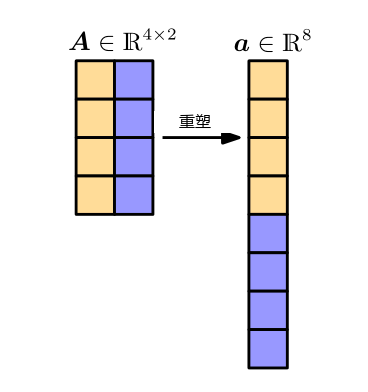
\includegraphics[width=320pt,keepaspectratio]{docs/images/Figure2.4.png}
\caption*{\refstepcounter{figcounter}\label{fig:2-4}图~\thefigcounter 通过堆叠其列，矩阵A可以表示为一个长向量a}
\end{figure}


\section*{2.2.1 矩阵加法和乘法}
\addcontentsline{toc}{subsection}{2.2.1 矩阵加法和乘法}

两个矩阵的和 $ \boldsymbol{A} \in \mathbb{R}^{m \times n}, \boldsymbol{B} \in \mathbb{R}^{m \times n} $ 被定义为对应元素的和，即，

\begin{equation}
\boldsymbol{A} + \boldsymbol{B} := \begin{bmatrix} a_{11} + b_{11} & \cdots & a_{1n} + b_{1n} \\ \vdots \\ a_{m1} + b_{m1} & \cdots & a_{mn} + b_{mn} \end{bmatrix} \in \mathbb{R}^{m \times n}
\tag{2.12}\label{eq:2-12}
\end{equation}

对于矩阵 $ \boldsymbol{A} \in \mathbb{R}^{m \times n}, \boldsymbol{B} \in \mathbb{R}^{n \times k} $ ，乘积 $ \boldsymbol{C} = \boldsymbol{A} \boldsymbol{B} \in \mathbb{R}^{m \times k} $ 的元素 $ c_{ij} $ 计算自

\begin{equation}
c_{ij} = \sum_{l=1}^{n}{a_{il}b_{lj}}, i = 1,...,m, \ j = 1,...,k
\tag{2.13}\label{eq:2-13}
\end{equation}

\begin{notebox}
注意矩阵的大小。
\end{notebox}

这意味着，为了计算元素 $ c_{ij} $，我们将 $ \boldsymbol{A} $ 的第 $ i $ 行的元素与 $ \boldsymbol{B} $ 的第 $ j $ 列的元素相乘，然后将它们相加。 稍后在第3.2节中，我们将称其为相应行和列的 \emph{点积（dot produc）} 。 在需要明确表示正在执行乘法的情况下，我们使用符号 $ \boldsymbol{A} \ · \boldsymbol{B} $  来表示乘法（明确显示“·”）。

\begin{notebox}
$ \boldsymbol{A} $ 中有 $ n $ 列，$ \boldsymbol{B} $ 中有 $ n $ 行，因此我们可以计算 $ a_{il}b_{lj} $，其中 $ l = 1,...,n $。 通常，两个向量 $ \boldsymbol{a}, \boldsymbol{b} $ 之间的点积表示为 $ \boldsymbol{a}^\top \boldsymbol{b} $ 或 $ \langle \boldsymbol{a}, \boldsymbol{b} \rangle $。
\end{notebox}

\emph{备注} 。 只有当它们的“相邻”维度匹配时，矩阵才能相乘。 例如，一个 $ n \times k $ 矩阵 $ \boldsymbol{A} $ 可以乘以一个 $ k \times m $ 矩阵 $ \boldsymbol{B} $ ，只能从左侧相乘：

\begin{equation}
\underbrace{\boldsymbol{A}}_{n \times k} \  \underbrace{\boldsymbol{B}}_{k \times m} = \underbrace{\boldsymbol{C}}_{n \times m}
\tag{2.14}\label{eq:2-14}
\end{equation}

如果 $ m \not= n $，则乘积  $ \boldsymbol {BA} $ 未定义，因为相邻维度不匹配。

\emph{备注} 。 矩阵乘法并非定义为矩阵逐元素的运算，即 $ c_{ij} \not= a_{ij}b_{ij} $（即使 $ \boldsymbol{A}\textcn{、}\boldsymbol{B} $ 的大小相同）。 当我们将（多维）数组彼此相乘时，这种逐元素乘法经常出现在编程语言中，称为 \emph{哈达玛乘积（Hadamard product）} 。

\begin{notebox}
\textbf{例 2.3}
\end{notebox}

\begin{notebox}
对于

\begin{equation*}
\boldsymbol{A} = \begin{bmatrix} 1 & 2 & 3 \\ 3 & 2 & 1 \end{bmatrix} \in \mathbb{R}^{2 \times 3}, \quad \boldsymbol{B} = \begin{bmatrix} 0 & 2 \\ 1 & -1 \\ 0 & 1 \end{bmatrix}  \in \mathbb{R}^{3 \times 2}
\end{equation*}

可以获得：

\begin{equation}
\boldsymbol {AB} = \begin{bmatrix} 1 & 2 & 3 \\ 3 & 2 & 1 \end{bmatrix} \begin{bmatrix} 0 & 2 \\ 1 & -1 \\ 0 & 1 \end{bmatrix} = \begin{bmatrix} 2 & 3\\ 2 & -5 \end{bmatrix} \in \mathbb{R}^{2 \times 2}
\tag{2.15}\label{eq:2-15}
\end{equation}

以及

\begin{equation}
\begin{adjustbox}{max width=\linewidth}
\boldsymbol {BA} = \begin{bmatrix} 0 & 2 \\ 1 & -1 \\ 0 & 1 \end{bmatrix} \begin{bmatrix} 1 & 2 & 3 \\ 3 & 2 & 1 \end{bmatrix} = \begin{bmatrix} 6 & 4 & 2\\ -2 & 0 & 2 \\ 3 & 2 & 1 \end{bmatrix} \in \mathbb{R}^{3 \times 3}
\end{adjustbox}
\tag{2.16}\label{eq:2-16}
\end{equation}
\end{notebox}

从这个例子中，我们已经可以看出矩阵乘法是不可交换的，即 $ \boldsymbol {AB} \not = \boldsymbol {BA} $； 另请参见图~\ref{fig:2-5} 中的说明。


\begin{figure}[H]
\centering
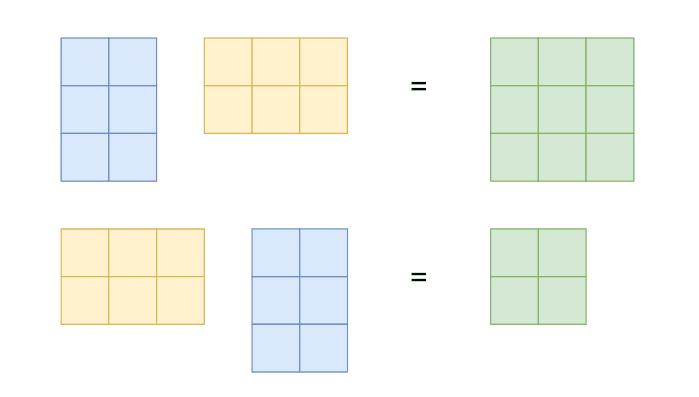
\includegraphics[width=0.92\textwidth,keepaspectratio]{docs/images/Figure2.5.png}
\caption*{\refstepcounter{figcounter}\label{fig:2-5}图~\thefigcounter 即使矩阵乘法 AB 和 BA 有意义，结果的维度也可能不同。}
\end{figure}


\textbf{定义 2.2} （单位矩阵）。 在 $ \mathbb{R}^{n \times n} $ 中，我们将 \emph{单位矩阵（identity matrix）} 定义为对角线上为 $ 1 $，其他地方为 $ 0 $ 的 $ n \times n $ 矩阵。

\begin{equation}
\begin{adjustbox}{max width=\linewidth}
\boldsymbol{I}_n :=  \begin{bmatrix} 1 & 0 & \cdots & 0 & \cdots & 0 \\ 0 & 1 & \cdots & 0 & \cdots & 0 \\ \vdots & \vdots & \ddots & \vdots & \ddots & \vdots \\ 0 & 0 & \cdots & 1 & \cdots & 0 \\ \vdots & \vdots & \ddots & \vdots & \ddots & \vdots \\ 0 & 0 & \cdots & 0 & \cdots & 1 \end{bmatrix} \in \mathbb{R}^{n \times n}
\end{adjustbox}
\tag{2.17}\label{eq:2-17}
\end{equation}

到目前我们定义了矩阵乘法、矩阵加法和单位矩阵，让我们看看矩阵的一些性质：

\begin{itemize}
\item 结合律：
\end{itemize}

\begin{equation}
\forall \boldsymbol{A} \in \mathbb{R}^{m \times n}, \ \boldsymbol{B} \in \mathbb{R}^{n \times p},\ \boldsymbol{C} \in \mathbb{R}^{p \times q} :\ (\boldsymbol{AB})\boldsymbol{C} = \boldsymbol{A} (\boldsymbol{BC})
\tag{2.18}\label{eq:2-18}
\end{equation}

\begin{itemize}
\item 交换律：
\end{itemize}

\begin{equation*}
\forall \boldsymbol {A,B} \in \mathbb{R}^{m \times n}, \ \boldsymbol {C,D} \in \mathbb{R}^{n \times p}:
\end{equation*}

\begin{equation}
(\boldsymbol{A} + \boldsymbol{B})\boldsymbol{C} = \boldsymbol{AC} + \boldsymbol{BC}
\tag{2.19a}\label{eq:2-19a}
\end{equation}

\begin{equation}
\boldsymbol{A} (\boldsymbol{C} + \boldsymbol{D}) = \boldsymbol{AC} + \boldsymbol{AD}
\tag{2.19b}\label{eq:2-19b}
\end{equation}

\begin{itemize}
\item 与单位矩阵相乘：
\end{itemize}

\begin{equation}
\forall \boldsymbol{A} \in \mathbb{R}^{m \times n}: \ \boldsymbol {I_m A} = \boldsymbol {A I_n} = \boldsymbol{A}
\tag{2.20}\label{eq:2-20}
\end{equation}

请注意，对于 $ m \not = n $，$ \boldsymbol{I}_m \not = \boldsymbol{I}_n $

\section*{2.2.2 逆和转置}
\addcontentsline{toc}{subsection}{2.2.2 逆和转置}

\textbf{定义 2.3} （逆）。对于一个方阵 $ \boldsymbol{A} \in \mathbb{R}^{n \times n} $，令矩阵 $ \boldsymbol{B} \in \mathbb{R}^{n \times n} $ 具有 $ \boldsymbol {AB} = \boldsymbol{I}_n = \boldsymbol {BA} $ 的性质。 $ \boldsymbol{B} $ 称为 $ \boldsymbol{A} $ 的 \emph{逆（inverse）} ，用 $ \boldsymbol{A}^{-1} $ 表示。

\begin{notebox}
方阵具有相同的列数和行数。
\end{notebox}

不幸的是，并非每个矩阵 $ \boldsymbol{A} $ 都具有逆 $ \boldsymbol{A}^{-1} $。 如果这个逆确实存在，则 A 称为 \emph{正则/可逆/非奇异（regular/invertible/nonsingular）} ，否则称为 \emph{奇异/不可逆（singular/noninvertible）} 。 当矩阵逆存在时，它是唯一的。 在 2.3 节中，我们将讨论通过求解线性方程组来计算矩阵逆的一般方法。

\emph{备注} （存在 2 × 2 矩阵的逆矩阵）。 考虑一个矩阵:

\begin{equation}
\boldsymbol{A} := \begin{bmatrix} a_{11} & a_{12} \\ a_{21} & a_{22} \end{bmatrix} \in \mathbb{R}^{2 \times 2}
\tag{2.21}\label{eq:2-21}
\end{equation}

如果我们将 $ \boldsymbol{A} $ 乘以

\begin{equation}
\boldsymbol{A}^{'} := \begin{bmatrix} a_{22} & -a_{12} \\ -a_{21} & a_{11} \end{bmatrix}
\tag{2.22}\label{eq:2-22}
\end{equation}

我们得到

\begin{equation}
\boldsymbol {AA^{'}} = \begin{bmatrix} a_{11}a_{22} - a_{12}a_{21} & 0 \\ 0 & a_{11}a_{22} - a_{12}a_{21} \end{bmatrix} = a_{11}a_{22} \boldsymbol{I}
\tag{2.23}\label{eq:2-23}
\end{equation}

因此

\begin{equation}
\boldsymbol{A}^{-1} =  \frac{1}{a_{11}a_{22} - a_{12}a_{21}}\begin{bmatrix} a_{22} & -a_{12} \\ -a_{21} & a_{11} \end{bmatrix}
\tag{2.24}\label{eq:2-24}
\end{equation}

当且仅当 $ a_{11}a_{22} - a_{12}a_{21} \not= 0 $。在4.1节中，我们将看到 $ a_{11}a_{22} - a_{12}a_{21} $ 是 2×2 矩阵的行列式。 此外，我们通常可以使用行列式来检查矩阵是否可逆。

\begin{notebox}
\textbf{例 2.4（逆矩阵）}
\end{notebox}

\begin{notebox}
矩阵

\begin{equation}
\begin{adjustbox}{max width=\linewidth}
\boldsymbol{A} = \begin{bmatrix} 1 & 2 & 1 \\ 4 & 4 & 5 \\ 6 & 7 & 7 \end{bmatrix}, \quad \boldsymbol{B} = \begin{bmatrix} -7 & -7 & 6 \\ 2 & 1 & -1 \\ 4 & 5 & -4 \end{bmatrix}
\end{adjustbox}
\tag{2.25}\label{eq:2-25}
\end{equation}

互为逆矩阵，因为 $ \boldsymbol {AB} = \boldsymbol{I} = \boldsymbol {BA} $。
\end{notebox}

\textbf{定义 2.4} （转置）。对于 $ \boldsymbol{A} \in \mathbb{R}^{m \times n} $，矩阵 $ \boldsymbol{B} \in \mathbb{R}^{n \times m} $ 且 $ b_{ij} = a_{ji} $ 称为 $ \boldsymbol{A} $ 的 \emph{转置（transpose）} 。 我们写 $ \boldsymbol{B} = \boldsymbol{A}^{\top} $。

一般情况下，可以通过将 $ \boldsymbol{A} $ 的列写为 $ \boldsymbol{A}^{\top} $ 的行来获得 $ \boldsymbol{A}^{\top} $ 。以下是逆和转置的重要性质：

\begin{equation}
\boldsymbol {AA^{-1}} = \boldsymbol{I} = \boldsymbol {A^{-1}A}
\tag{2.26}\label{eq:2-26}
\end{equation}

\begin{equation}
\boldsymbol {(AB)^{-1}} = \boldsymbol {B^{-1}A^{-1}}
\tag{2.27}\label{eq:2-27}
\end{equation}

\begin{equation}
\boldsymbol {(A + B)^{-1}} \not= \boldsymbol {A^{-1} + B^{-1}}
\tag{2.28}\label{eq:2-28}
\end{equation}

\begin{equation}
(\boldsymbol {A^{\top})^{\top}} = \boldsymbol{A}
\tag{2.29}\label{eq:2-29}
\end{equation}

\begin{equation}
\boldsymbol {(A + B)^{\top}} = \boldsymbol {A^{\top} + B^{\top}}
\tag{2.30}\label{eq:2-30}
\end{equation}

\begin{equation}
\boldsymbol {(AB)^{\top}} = \boldsymbol {B^{\top}A^{\top}}
\tag{2.31}\label{eq:2-31}
\end{equation}

\begin{notebox}
矩阵 $ \boldsymbol{A} $ 的主对角线是全部 $ A_{ij} $ 的集合，其中 $ i = j $。 (2.28) 的标量情况是 $ \frac{1}{2 + 4} = \frac{1}{6} \not= \frac{1}{2} + \frac{1}{6} $
\end{notebox}

\textbf{定义 2.5} （对称矩阵）。如果 $ \boldsymbol{A} = \boldsymbol{A}^{\top} $， 则矩阵 $ \boldsymbol{A} \in \mathbb{R}^{n \times n} $ 是 \emph{对称矩阵（symmetric matrix）} 。

请注意，只有 $ (n, n) $ 矩阵才可以是对称的。通常，我们称 $ (n, n) $ 矩阵也为 \emph{方阵（square matrix）} ，因为它们具有相同的行数和列数。此外，如果 $ \boldsymbol{A} $ 是可逆的，那么 $ \boldsymbol{A}^{\top} $ 也是可逆的，并且 $ (\boldsymbol{A}^{-1})^{\top} = (\boldsymbol{A}^{\top})^{-1} =: \boldsymbol{A}^{\top} $ 。

\emph{备注} （对称矩阵的和与乘积）。 对称矩阵  $ \boldsymbol {A,B} \in \mathbb{R}^{n \times n} $ 的总和总是对称的。 然而，虽然他们的乘积有意义，但它通常不是对称的：

\begin{equation}
\begin{bmatrix} 1 & 0 \\ 0 & 0 \end{bmatrix} \begin{bmatrix} 1 & 1 \\ 1 & 1 \end{bmatrix} = \begin{bmatrix} 1 & 1 \\ 0 & 0 \end{bmatrix}
\tag{2.32}\label{eq:2-32}
\end{equation}

\section*{2.2.3 乘以标量}
\addcontentsline{toc}{subsection}{2.2.3 乘以标量}

让我们看看当矩阵乘以标量 $ \lambda \in \mathbb{R} $ 时会发生什么。让 $ \boldsymbol{A} \in \mathbb{R}^{m \times n} $ 和 $ \lambda \in \mathbb{R} $，然后 $ \lambda \boldsymbol{A} =  \boldsymbol{K}, K_{ij} = \lambda a_{ij} $ 。 实际上， $ \lambda $ 缩放了 $ \boldsymbol{A} $ 的每个元素。 对于 $ \lambda,\psi \in \mathbb{R} $，以下成立：

\begin{itemize}
\item 结合律 
\end{itemize}

\begin{equation*}
(\lambda \psi)\boldsymbol{C} = \lambda(\psi \boldsymbol{C}), \ \boldsymbol{C} \in \mathbb{R}^{m \times n}
\end{equation*}

\begin{itemize}
\item 。请注意，这意味着我们可以随意移动标量值。
\end{itemize}
\begin{equation*}
\begin{adjustbox}{max width=\linewidth}
\lambda (\boldsymbol {BC}) = (\lambda \boldsymbol{B}) \boldsymbol{C} = \boldsymbol{B} (\lambda \boldsymbol{C}) = (\boldsymbol {BC}) \lambda, \ \boldsymbol{B} \in \mathbb{R}^{m \times n}, \  \boldsymbol{C} \in \mathbb{R}^{n \times k}
\end{adjustbox}
\end{equation*}
\begin{itemize}
\end{itemize}

\begin{itemize}
\item $ (\lambda \boldsymbol{C})^{\top} = \boldsymbol{C}^{\top} \lambda^{\top} = \boldsymbol{C}^{\top} \lambda = \lambda \boldsymbol{C}^{\top} $ ， 因为对于所有的 $ \lambda \in \mathbb{R}, \ \lambda = \lambda^{\top} $ 。
\end{itemize}

\begin{itemize}
\item 分配律 
\end{itemize}

\begin{equation*}
(\lambda + \psi) \boldsymbol{C} = \lambda \boldsymbol{C} + \psi \boldsymbol{C}, \ \boldsymbol{C} \in \mathbb{R}^{m \times n}
\end{equation*}

\begin{equation*}
\lambda (\boldsymbol{B} + \boldsymbol{C}) = \lambda \boldsymbol{B} + \lambda \boldsymbol{C}, \ \boldsymbol {B,C} \in \mathbb{R}^{m \times n}
\end{equation*}

\begin{notebox}
\textbf{例 2.5（分配律）}
\end{notebox}

\begin{notebox}
如果我们定义

\begin{equation}
\boldsymbol{C} := \begin{bmatrix} 1 & 2 \\ 3 & 4 \end{bmatrix}
\tag{2.33}\label{eq:2-33}
\end{equation}

那么对于任何 $ \lambda, \psi \in \mathbb{R} $，我们得到：

\begin{equation}
\begin{adjustbox}{max width=\linewidth}
(\lambda + \psi)\boldsymbol{C} = \begin{bmatrix} (\lambda + \psi)1 & (\lambda + \psi)2 \\ (\lambda + \psi)3 & (\lambda + \psi)4 \end{bmatrix} = \begin{bmatrix} \lambda + \psi & 2\lambda + 2\psi \\ 3\lambda + 3\psi & 4\lambda + 4\psi \end{bmatrix}
\end{adjustbox}
\tag{2.34a}\label{eq:2-34a}
\end{equation}

\begin{equation}
= \begin{bmatrix} \lambda & 2\lambda \\ 3\lambda & 4\lambda \end{bmatrix} + \begin{bmatrix} \psi & 2\psi \\ 3\psi & 4\psi \end{bmatrix} = \lambda \boldsymbol{C} + \psi \boldsymbol{C}
\tag{2.34b}\label{eq:2-34b}
\end{equation}
\end{notebox}

\section*{2.2.4 线性方程组的紧凑表示}
\addcontentsline{toc}{subsection}{2.2.4 线性方程组的紧凑表示}

如果我们考虑线性方程组

\begin{equation}
2x_1 + 3x_2 + 5x_3 = 1 \\
4x_1 - 2x_2 - 7x_3 = 8 \\
9x_1 + 5x_2 - 3x_3 = 2
\tag{2.35}\label{eq:2-35}
\end{equation}

并使用矩阵乘法的规则，我们可以将这个方程组写成更紧凑的形式

\begin{equation}
\begin{bmatrix} 2 & 3 & 5 \\ 4 & -2 & -7 \\ 9 & 5 & -3 \end{bmatrix} \begin{bmatrix} x_1 \\ x_2 \\ x_3 \end{bmatrix} = \begin{bmatrix} 1 \\ 8 \\ 2 \end{bmatrix}
\tag{2.36}\label{eq:2-36}
\end{equation}

请注意，$ x_1 $ 缩放第一列，$ x_2 $ 缩放第二列，$ x_3 $ 缩放第三列。

通常，线性方程组可以用其矩阵形式紧凑地表示为 $ \boldsymbol {Ax} = \boldsymbol{b} $； 见 (2.3)，乘积 $ \boldsymbol {Ax} $ 是 $ \boldsymbol{A} $ 的列的（线性）组合。 我们将在 2.5 节中更详细地讨论线性组合。
